\chapter{Abalone}
\label{abalone}
Abalone was devised by Michel Lalet and Laurent Lévi. Even though it was created fairly recently, more than four million global sales have established Abalone as a classic game \cite{noauthor_abalone_2020}.

\section{Rules}

\begin{figure}[!h]
    \centering
    \subfloat[Starting position]{
        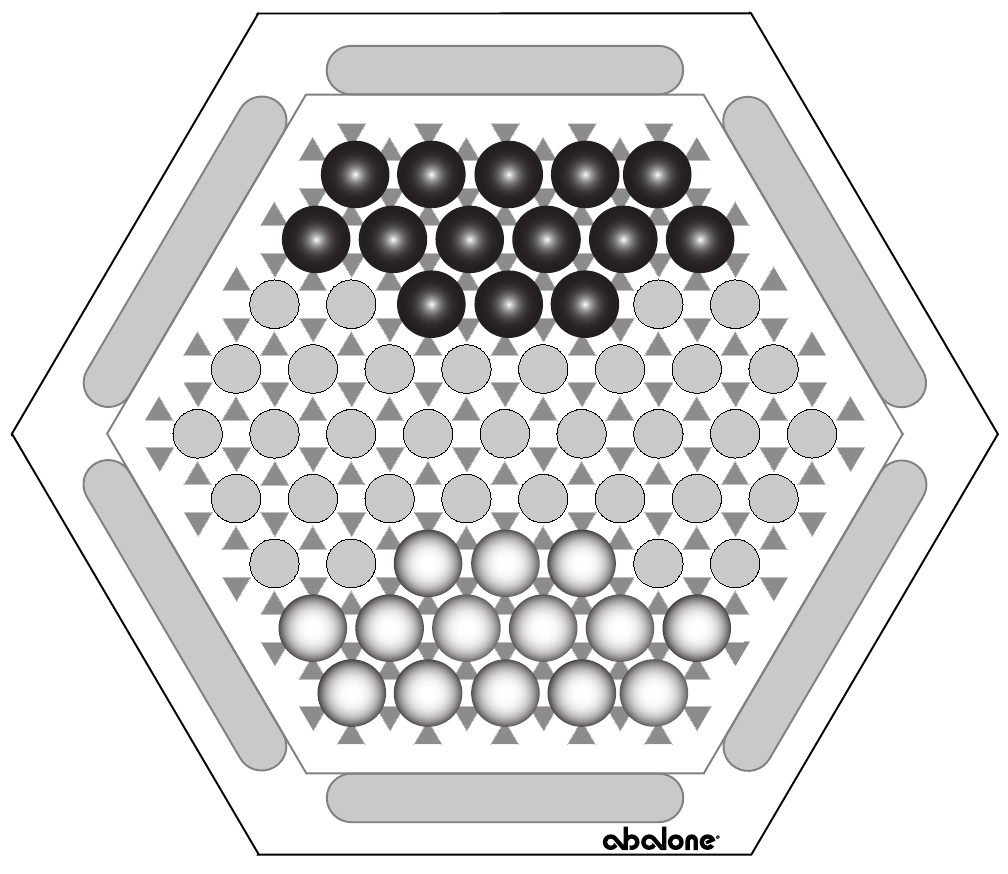
\includegraphics[width=4.5cm, keepaspectratio]{rules_starting_position.png}
    }
    \hfill
    \subfloat["In-line" moves]{
        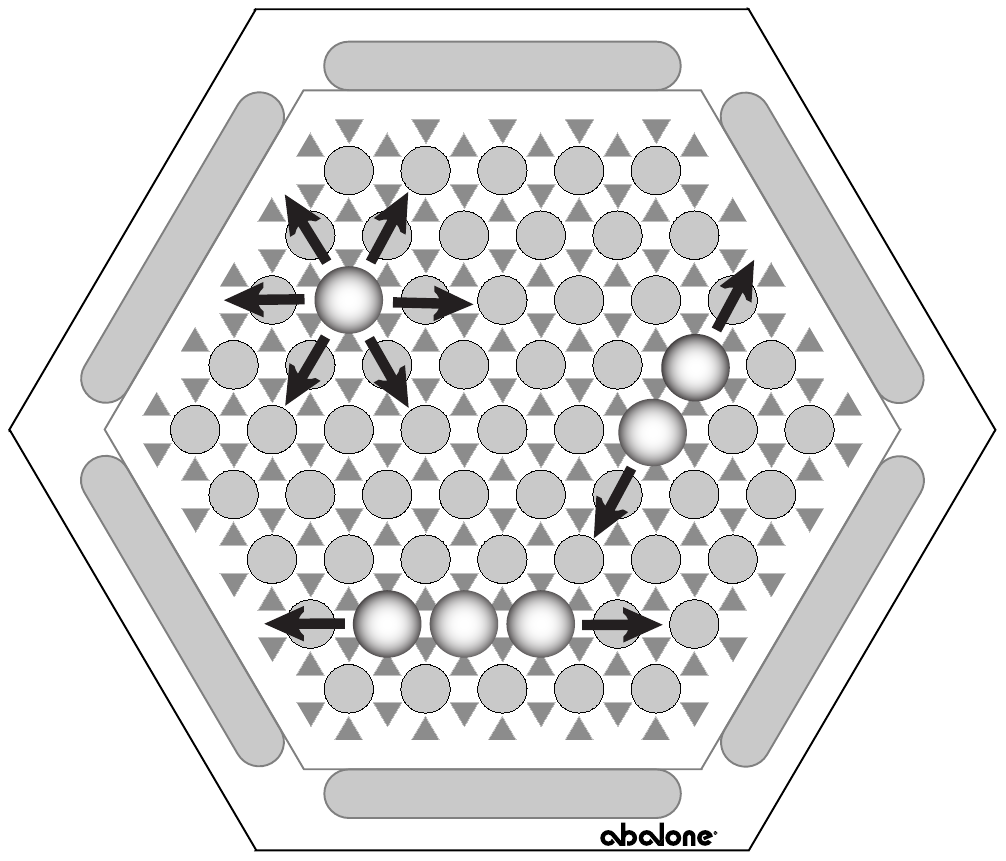
\includegraphics[width=4.5cm, keepaspectratio]{rules_inline_move.png}
    }
    \hfill
    \subfloat["Side-step" moves]{
        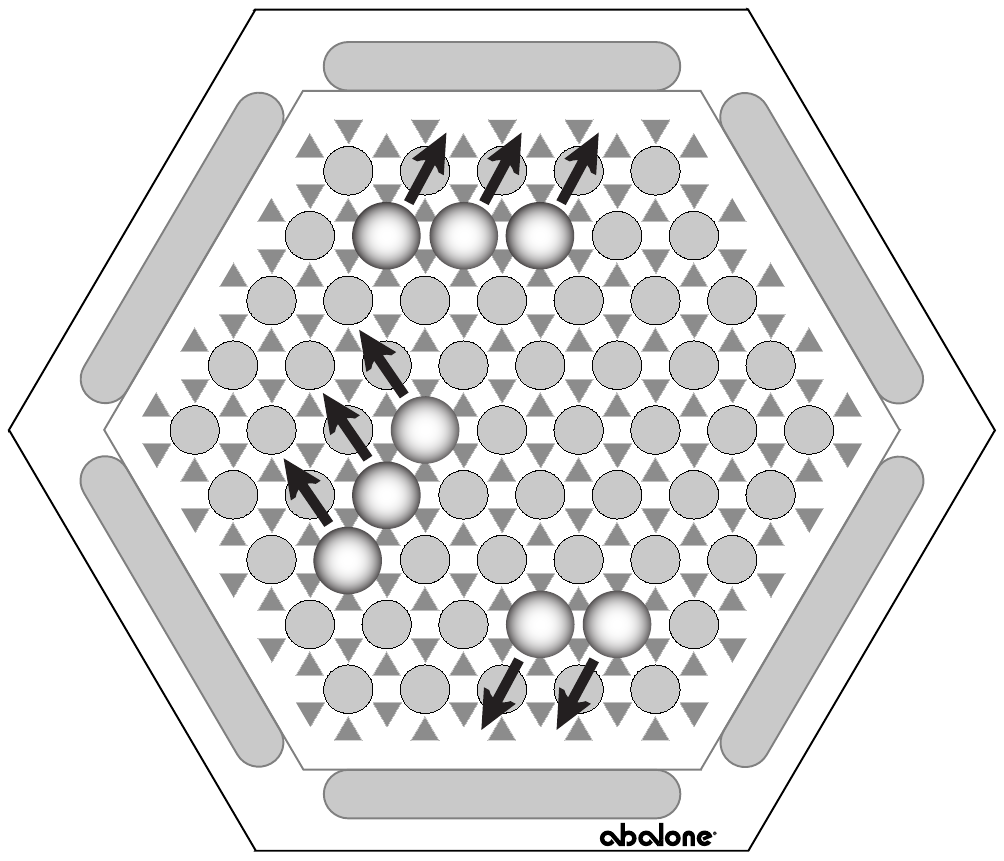
\includegraphics[width=4.5cm, keepaspectratio]{rules_side_step_move.png}
    }
    \caption{Basic moves \cite{abalone_sa_abalone_nodate}}
    \label{basics}
\end{figure}

In the classical variant, each player places 14 marbles on opposing sides. Figure \ref{basics} (a) depicts the game's default starting position. Other starting positions like "German daisy" and "Belgian daisy" and four-player variants will not be considered. The player may move one, two, or three adjacent marbles in one of the six possible directions. The marbles have to move in the same direction and only move to a neighboring field. We differentiate between broadside or "side-step" moves and "in-line" moves, depending on how the chain of marbles moves relative to its direction. The difference is shown in figure \ref{basics} (b) and (c).

\begin{figure}[!h]
    \centering
    \subfloat["2-push-1" sumito]{
        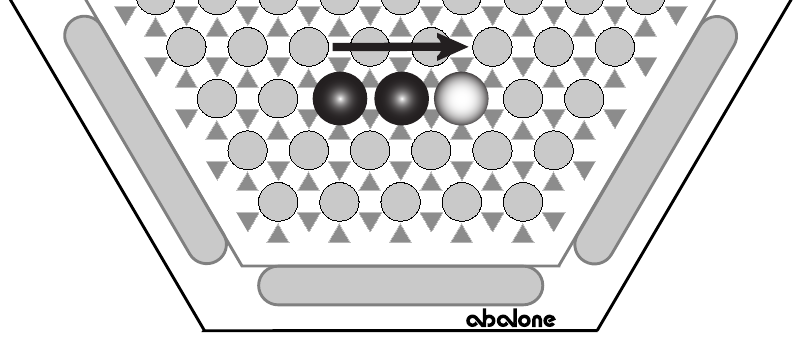
\includegraphics[width=4.5cm, keepaspectratio]{rules_2-push-1_sumito.png}
    }
    \hfill
    \subfloat["3-push-1" sumito]{
        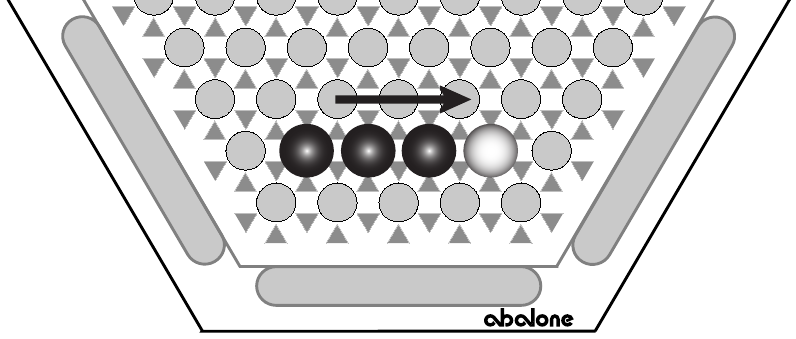
\includegraphics[width=4.5cm, keepaspectratio]{rules_3-push-1_sumito.png}
    }
    \hfill
    \subfloat["3-push-2" sumito]{
        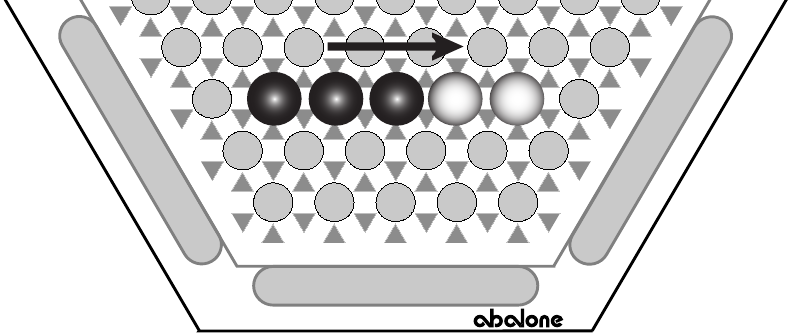
\includegraphics[width=4.5cm, keepaspectratio]{rules_3-push-2_sumito.png}
    }
    \caption{Sumito positions allow pushing the opponent's marbles \cite{abalone_sa_abalone_nodate}}
    \label{sumito}
\end{figure}

A move pushing the opponent's marbles is called "sumito" and comes in three variations, as shown by figure \ref{sumito}. Essentially, the player has to push with superior numbers.

\begin{figure}[!h]
    \centering
    \subfloat[Different blocking situations]{
        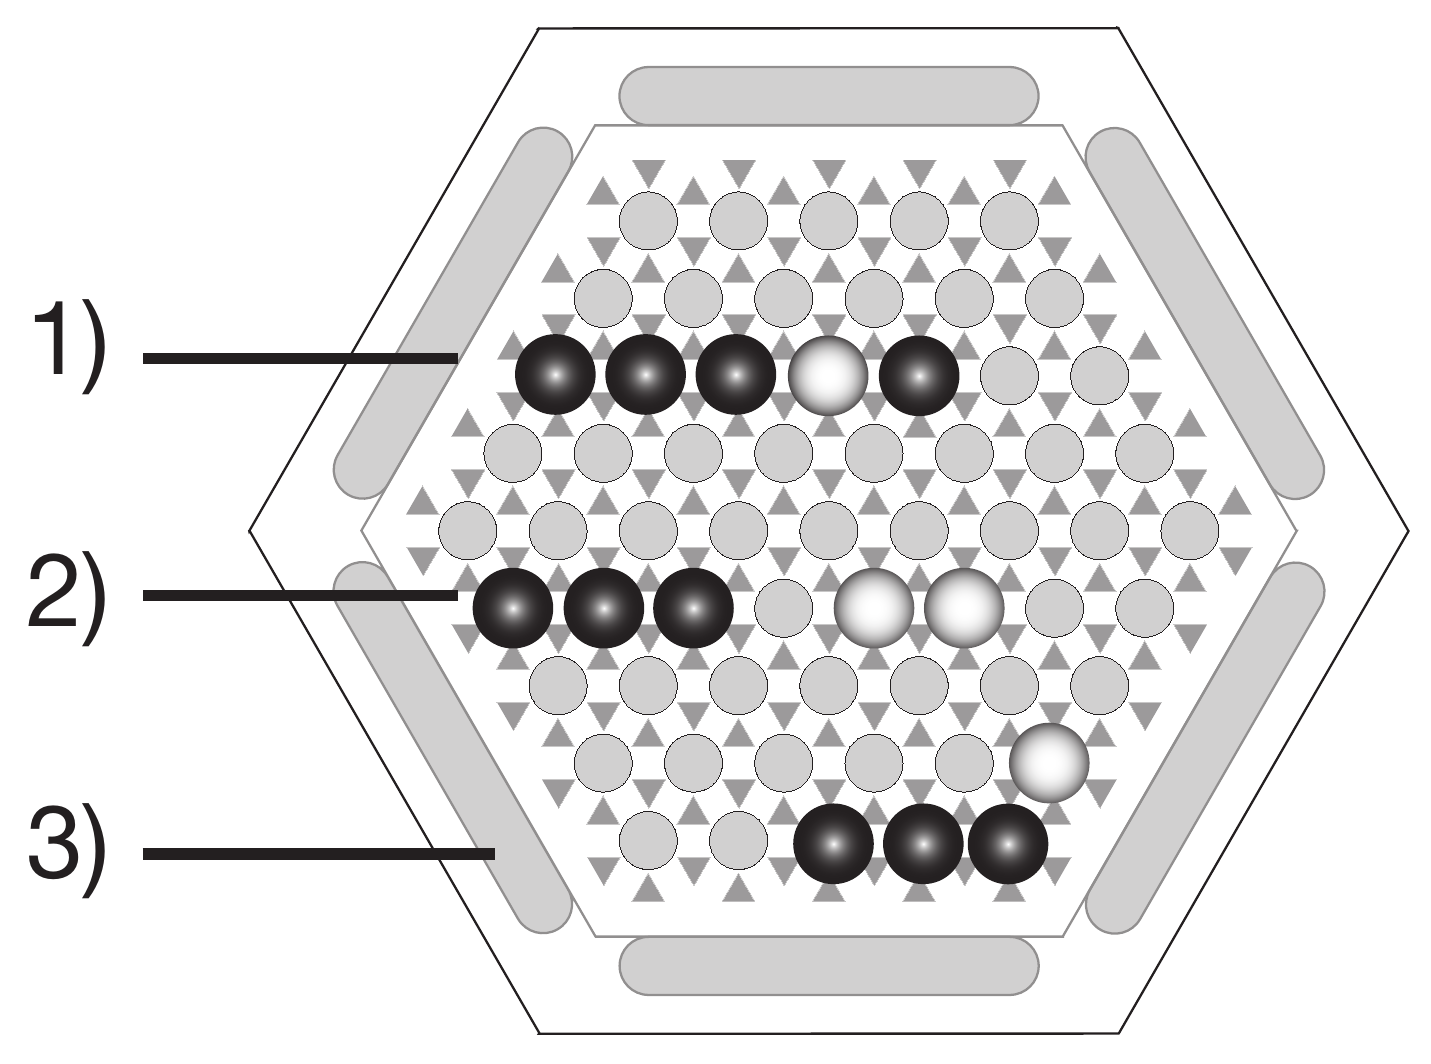
\includegraphics[width=4.5cm, keepaspectratio]{rules_block.png}
    }
    \hfill
    \subfloat[Attacking position]{
        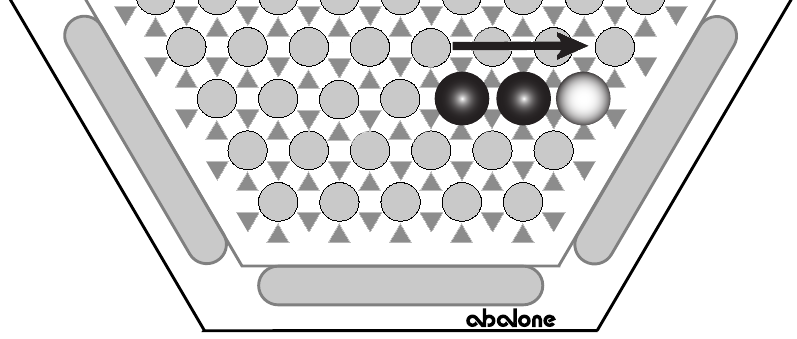
\includegraphics[width=4.5cm, keepaspectratio]{rules_attacking_move.png}
    }
    \hfill
    \subfloat[No legal move available to black]{
        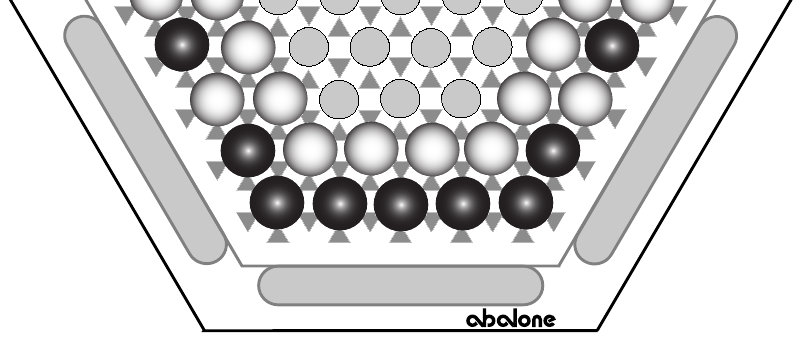
\includegraphics[width=4.5cm, keepaspectratio]{rules_stalemate.png}
    }
    \caption{Additional relevant board positions \cite{abalone_sa_abalone_nodate}}
    \label{additional_relevant_positions}
\end{figure}

A sumito might be blocked by other marbles, as shown in figure  \ref{additional_relevant_positions} (a). In 1) the sumito by black is blocked by the black marble, in 2) there is a free space between the marbles, and 3) shows how a side-step cannot push a marble. Sumito moves are the only moves that allow for pushing the enemy's marbles. Therefore, they are the only attacking moves. Figure \ref{additional_relevant_positions} (b) shows a situation in which we can push an enemy marble from the board. The player that pushes six of the opponent's marbles from the board has won. The basic ruleset does not account for a draw, but there are, in theory, positions like a stalemate in chess, where no move is possible for one player. In figure \ref{additional_relevant_positions} (c), the black player is locked to the brink of the board and has no move available. Moreover, to force a more eventful game, games are often limited by time or the number of moves. Thus, a draw might occur when the number of marbles left on the board is equal for each player.

\section{Task environment}
Based on the PEAS framework, we can specify Abalone as a task environment and show the key components for the implementation of our agent. \cite[p.107]{russell_artificial_2021}

\begin{description}
    \item[Performance measure] Win/loss, number of moves, time to deliberate
    \item[Environment] Digital playing board and rules of the game
    \item[Actuators] Move marbles
    \item[Sensors] Position of marbles
\end{description}

Using the environment properties learned in \ref{environment} we can classify Abalone as \textbf{a fully observable, deterministic, two-agent, competitive, sequential, static, and discrete environment}. Another popular term for this type of environment is a \textit{deterministic two-player turn-based perfect information zero-sum game}.

\section{Board Representations}
\label{board_representations}

There are multiple possible coordinate systems for the hexagonal boards to address the marble positions universally. In Abalone, the most common way is to label the rows alphabetically from A-I starting at the bottom row. The "columns" are labeled numerically from 1-9 as depicted in figure \ref{abalone_coordinate_systems} (a).

Cube coordinates, as proposed by Patel \cite{noauthor_red_nodate}, are a convenient way to represent hexagonal boards. The idea is to imagine a cube with a cartesian coordinate system originating from its center. At $x + y + z = 0$ a diagonal plane is sliced out resulting in the coordinate system represented in figure \ref{abalone_coordinate_systems} (b). It allows for the simpler application of a wide variety of formulas and algorithms like Manhattan distance, accessing neighbors, finding paths, etc., to the hexagonal board. Later, the cube coordinates will be utilized to calculate heuristics and to create symmetrical boards.

\begin{figure}[!h]
    \centering
    \subfloat[The most common coordinate system for Abalone]{
        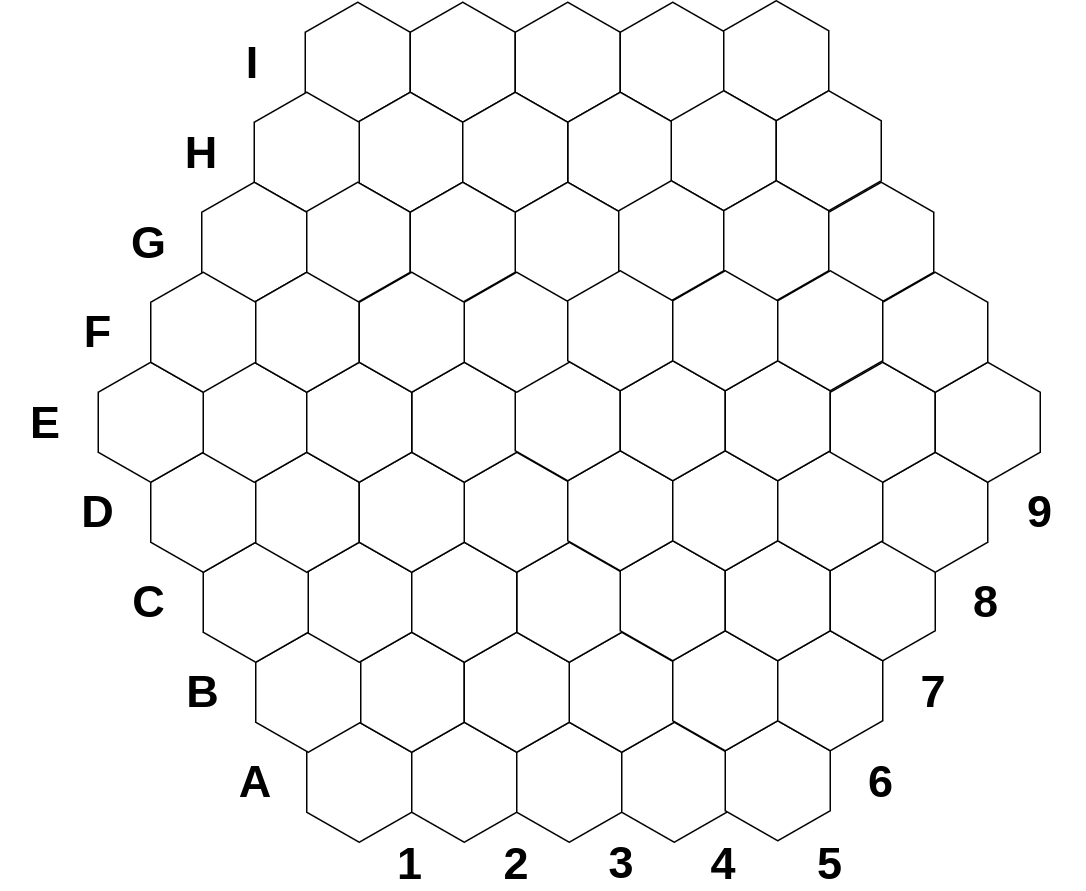
\includegraphics[height=6cm, keepaspectratio]{abalone_board_coordinates.png}
    }
    % \hfill
    \subfloat[The cube coordinate system \cite{noauthor_red_nodate}]{
        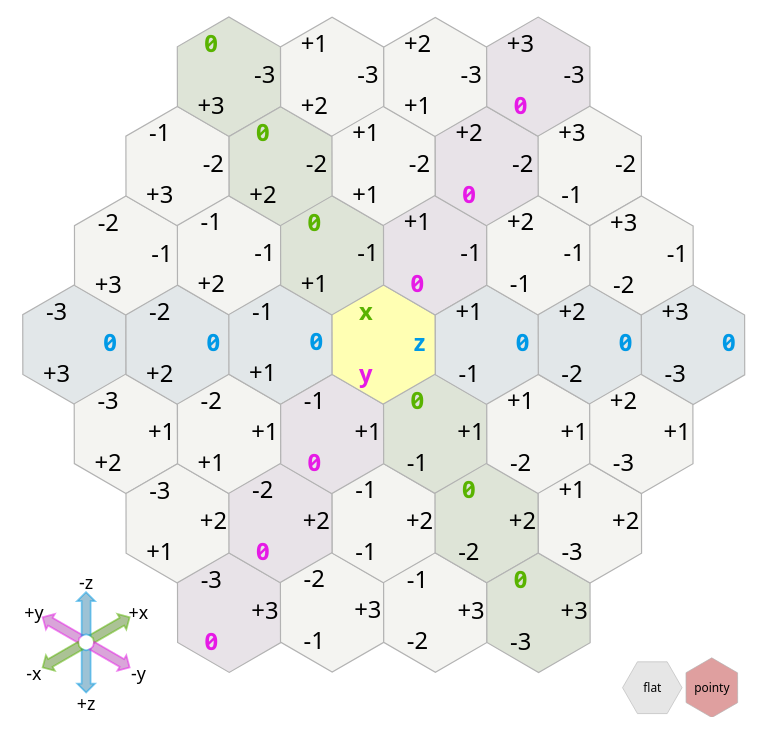
\includegraphics[height=6cm, keepaspectratio]{hex_cube_grid.png}
    }
    \caption{Different possibilities for addressing the fields of Abalone}
    \label{abalone_coordinate_systems}
\end{figure}

A different representation is advantageous to store the board state in a program or feed it to a neural network: Transforming the board into a two-dimensional array of integers. The players' marbles are represented as $1$ for black, $-1$ for white, and 0 for a space. As suggested by "towzeur" \cite{towzeur_towzeurgym-abalone_2021}, shifting the upper part of the board to the right creates an orthogonal basis. Therefore, the adjacency of the original hexagonal board is maintained.

\begin{figure}[!h]
    \centering
    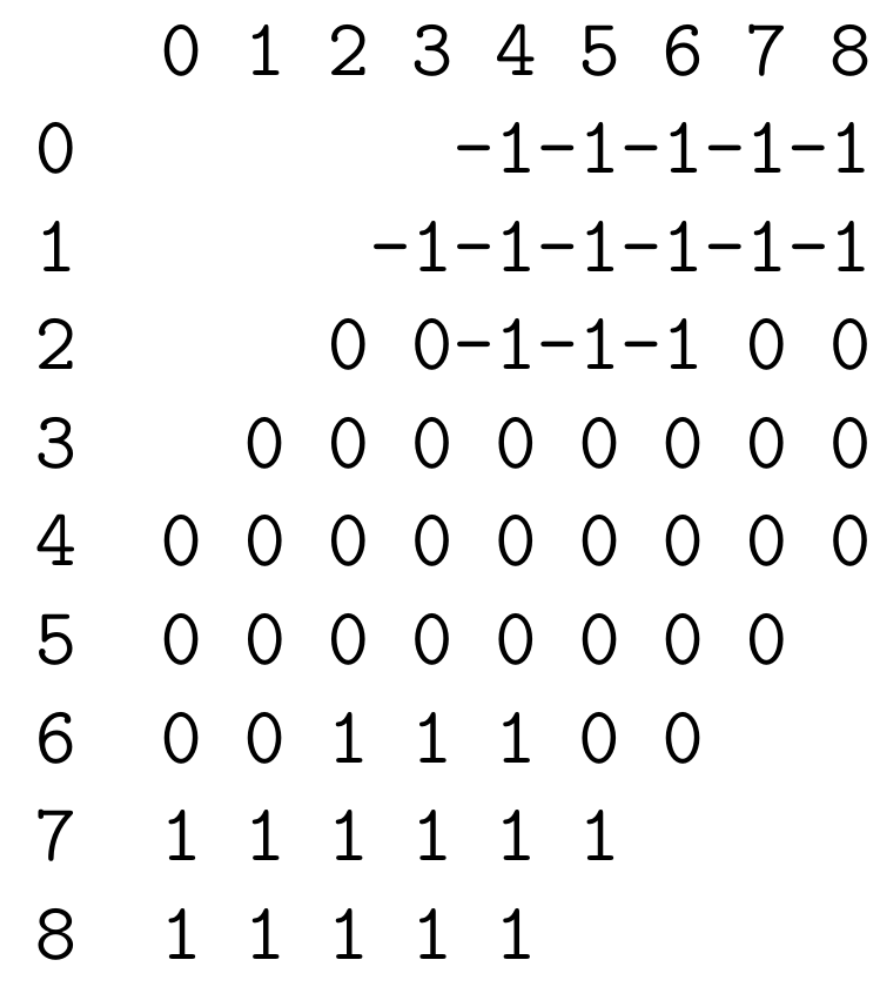
\includegraphics[height=6cm, keepaspectratio]{matrix_representation_white_turn.png}
    \caption{The matrix representation (the $0$ values for the corners of the matrix are ignored, for better visibility)}
    \label{abalone_matrix_representation}
\end{figure}

\section{Move notation}
\label{abalone_move_notation}
There is no officially standardized notation for the moves of Abalone. The notation described by Aichholzer \cite{aichholzer_abalone_2006} has wide adoption in the papers investigated. To contribute to the proliferation of standards \cite{xkcd_standards_nodate} we used a different notation that stems from the Abalone engine Abalone-BoAI \cite{scriptim_scriptimabalone-boai_2021}.

Inline moves have the structure of "\{MarbleCoordinate\}\{Direction\}" and broadside moves the structure of "\{MarbleCoordinate\}\{MarbleCoordinate\}\{Direction\}". Additionally, the marble coordinates are ordered for broadside moves. The marble coordinates have the form outlined in figure \ref{abalone_coordinate_systems} (a). The directions are always seen from the black player's starting position, north pointing straight in the direction of the white player (default position). This is the main difference to the notation described by Aichholzer, who uses a destination coordinate instead of a direction. The direction improves the readability and understandability of moves. The six directions are arranged just as in a compass, N for north, NW for north-west and so on. As follows, the regex for the notation:

\begin{BVerbatim}
    ([A-I][1-9]){1}([A-I][1-9]){0,1}((NE)|(E)|(SE)|(SE)|(SW)|(W)|(NW)){1}
\end{BVerbatim}

For example, an inline move with the marble at A1 as trailing marble in the direction north-east would be denoted as A1NE. A broadside move of a row of marbles from C3 until C5 in the direction of north-west would be denoted as C3C5NW.

\section{Symmetries}
\label{abalone_symmetries}

\begin{figure}
    \centering
    \subfloat[Mirror axes]{
        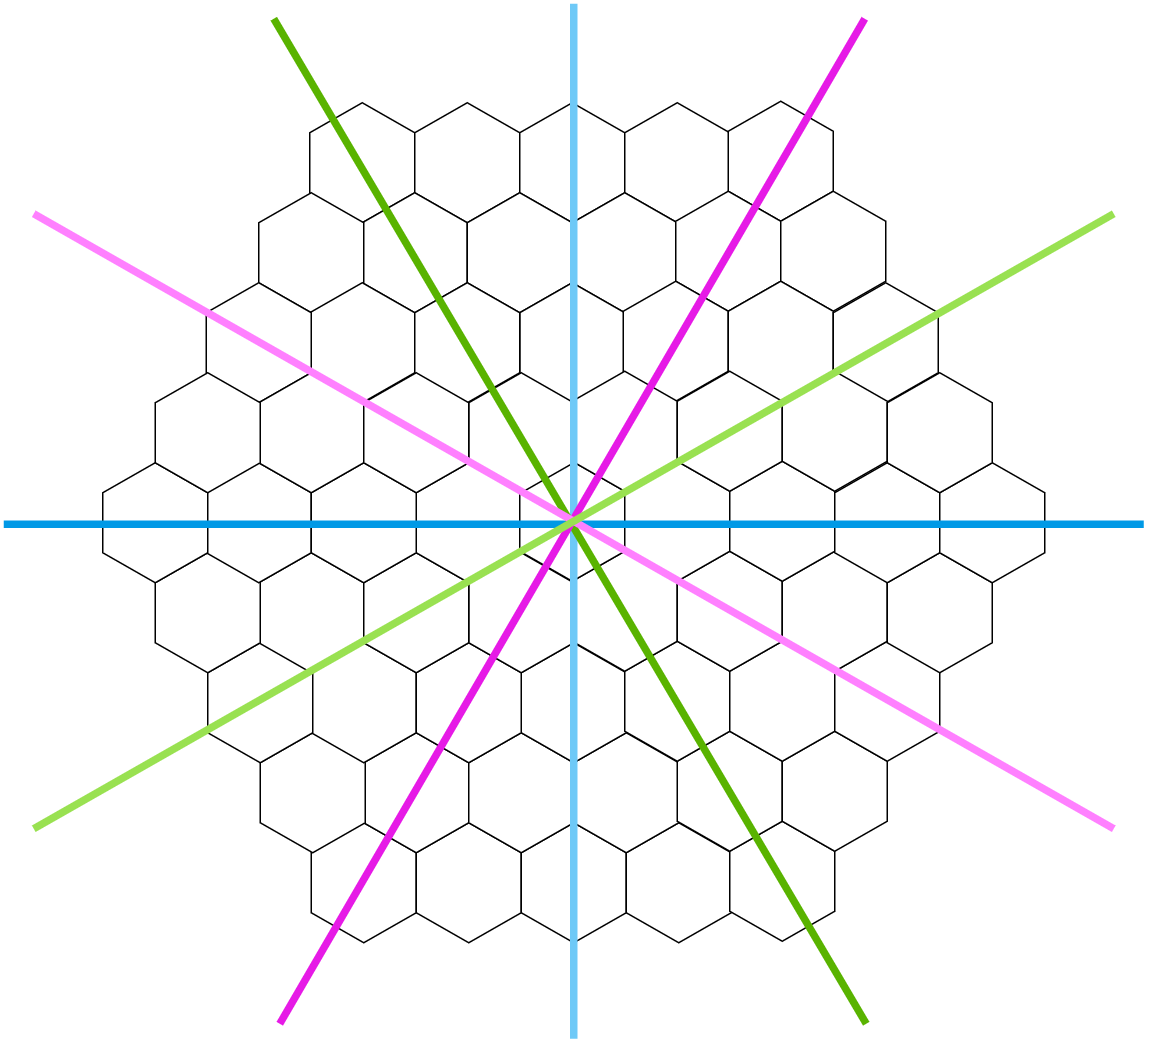
\includegraphics[height=6cm, keepaspectratio]{abalone_board_mirror_axes.png}
    }
    % \hfill
    \subfloat[Rotations]{
        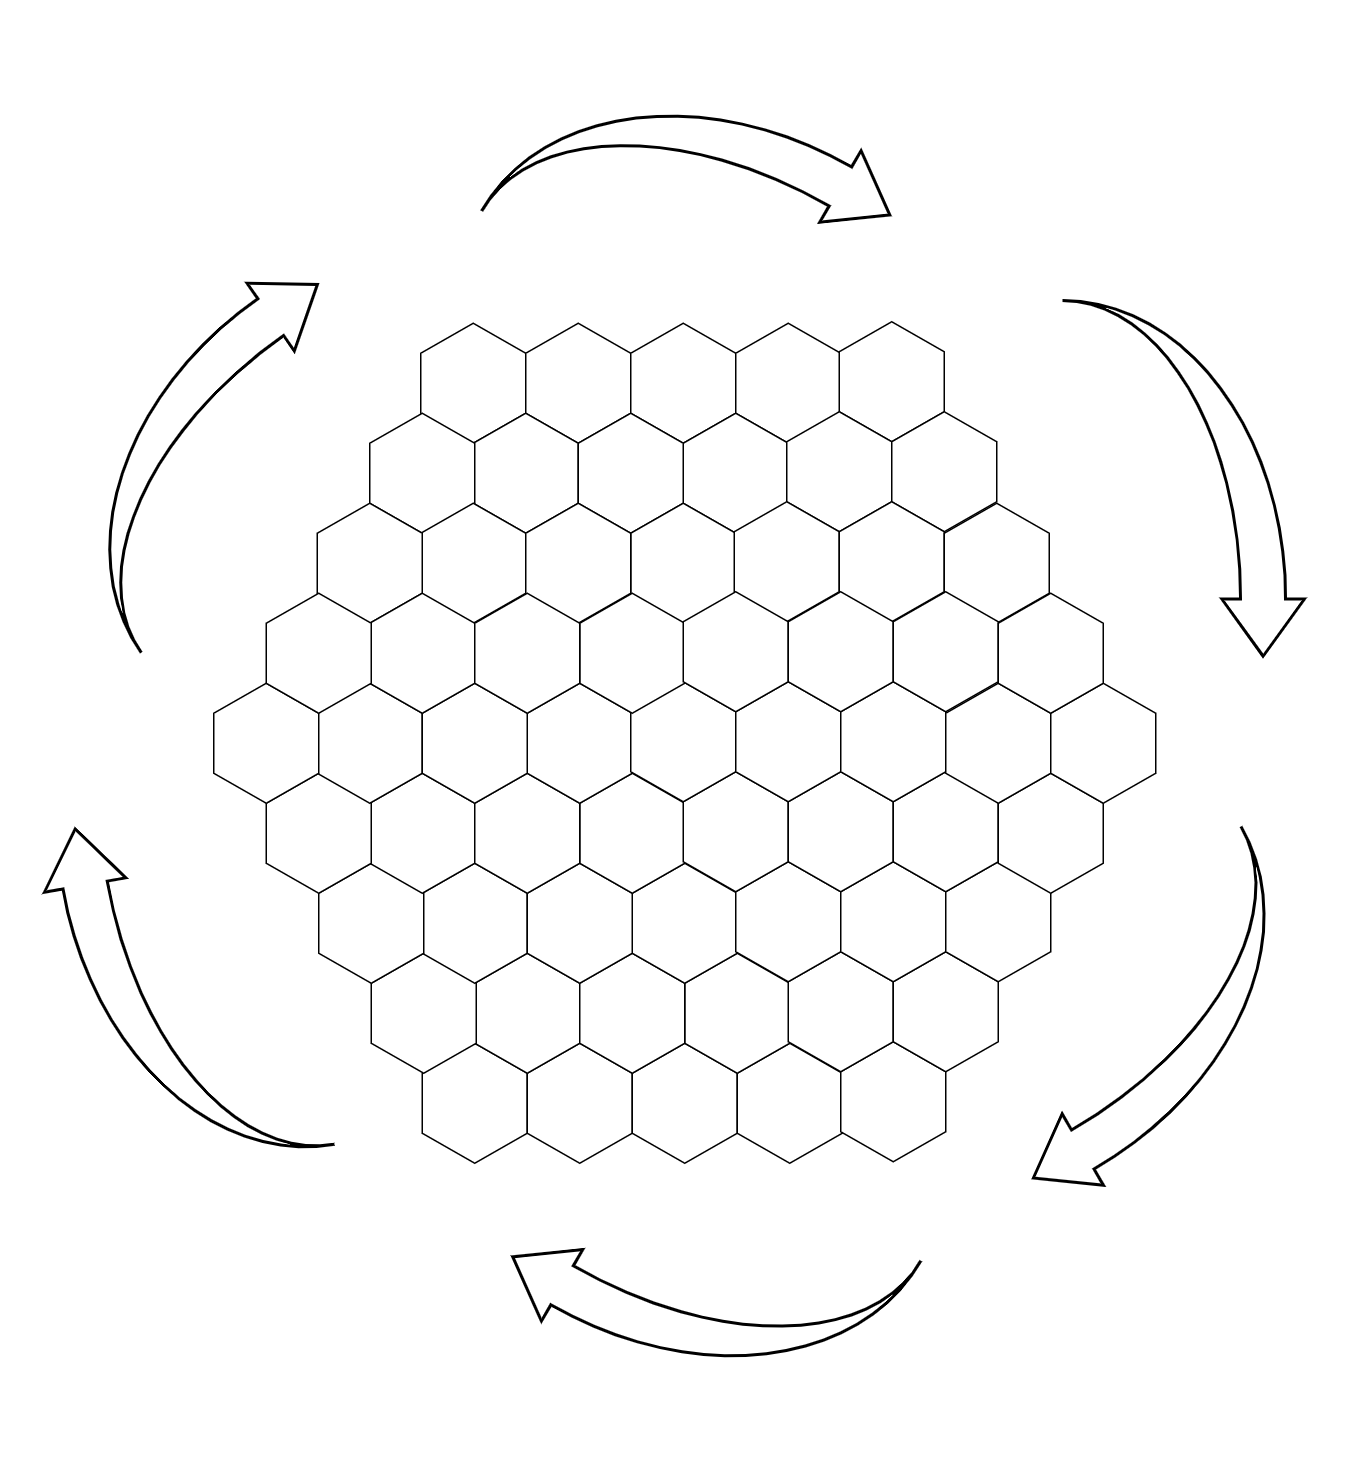
\includegraphics[height=7cm, keepaspectratio]{abalone_board_rotations.png}
    }
    \caption{The symmetries of the Abalone board}
    \label{abalone_symmetries_figure}
\end{figure}

The board of Abalone has six rotational symmetries and additional six mirror axes. There are three main axes $q, r, s$ that represent the coordinate basis shown in figure \ref{abalone_coordinate_systems} (b). Each of these has an additional orthogonal axis resulting in six distinct axes.

The rotations depicted in figure \ref{abalone_symmetries_figure} each describe a rotation by 60° clockwise.

\section{Complexity}
As Abalone has a finite amount of discrete states, we can make precise statements about its complexity, which one can describe in two relevant dimensions.

\paragraph{State space complexity}
\label{state_space_complexity}

The state space is the set of all possible states "the environment can be in." \cite[p. 150]{russell_artificial_2021} For Abalone, this means we have to consider all possible board configurations with different numbers of marbles present. Additionally, duplicates that arise from the symmetries of the board have to be removed. The following formula gives us a good upper bound:

\begin{equation}
    \sum_{k=8}^{14}\sum_{m=9}^{14}\frac{61!}{k!(61-k)!}\cdot\frac{(61-k)!}{m!((61-k)-m)!}
\end{equation}

Due to the board's symmetries,the results have to be divided by 12 which results in a total of $ 6 \cdot 10^{23} $ possible board configurations. \cite[p. 4]{lemmens_constructing_2005}

\paragraph{Game tree complexity} Abalone's game tree is unbound and has an infinite height as actions might be taken repeatedly, forming loops. Therefore, Abalone's complexity is not determined by the game tree but is approximated by an average search tree. First, we consider the branching factor $ b $, or the number of possible moves for any given state. This number greatly varies between different states. On average Abalone has $ b = 60 $ possible moves per state as measured in figure \ref{branching_factor}. The depth $ d $ of the tree depends on the number of turns per game. The average game takes approximately $ d = 87 $ turns. The number of nodes in a tree gives a measure of the complexity:

\begin{equation}
    b^d
\end{equation}

resulting in a total of $60^{87} \approx 5 \cdot 10^{154}$ nodes. \cite{lemmens_constructing_2005}

\begin{figure}
    \centering
    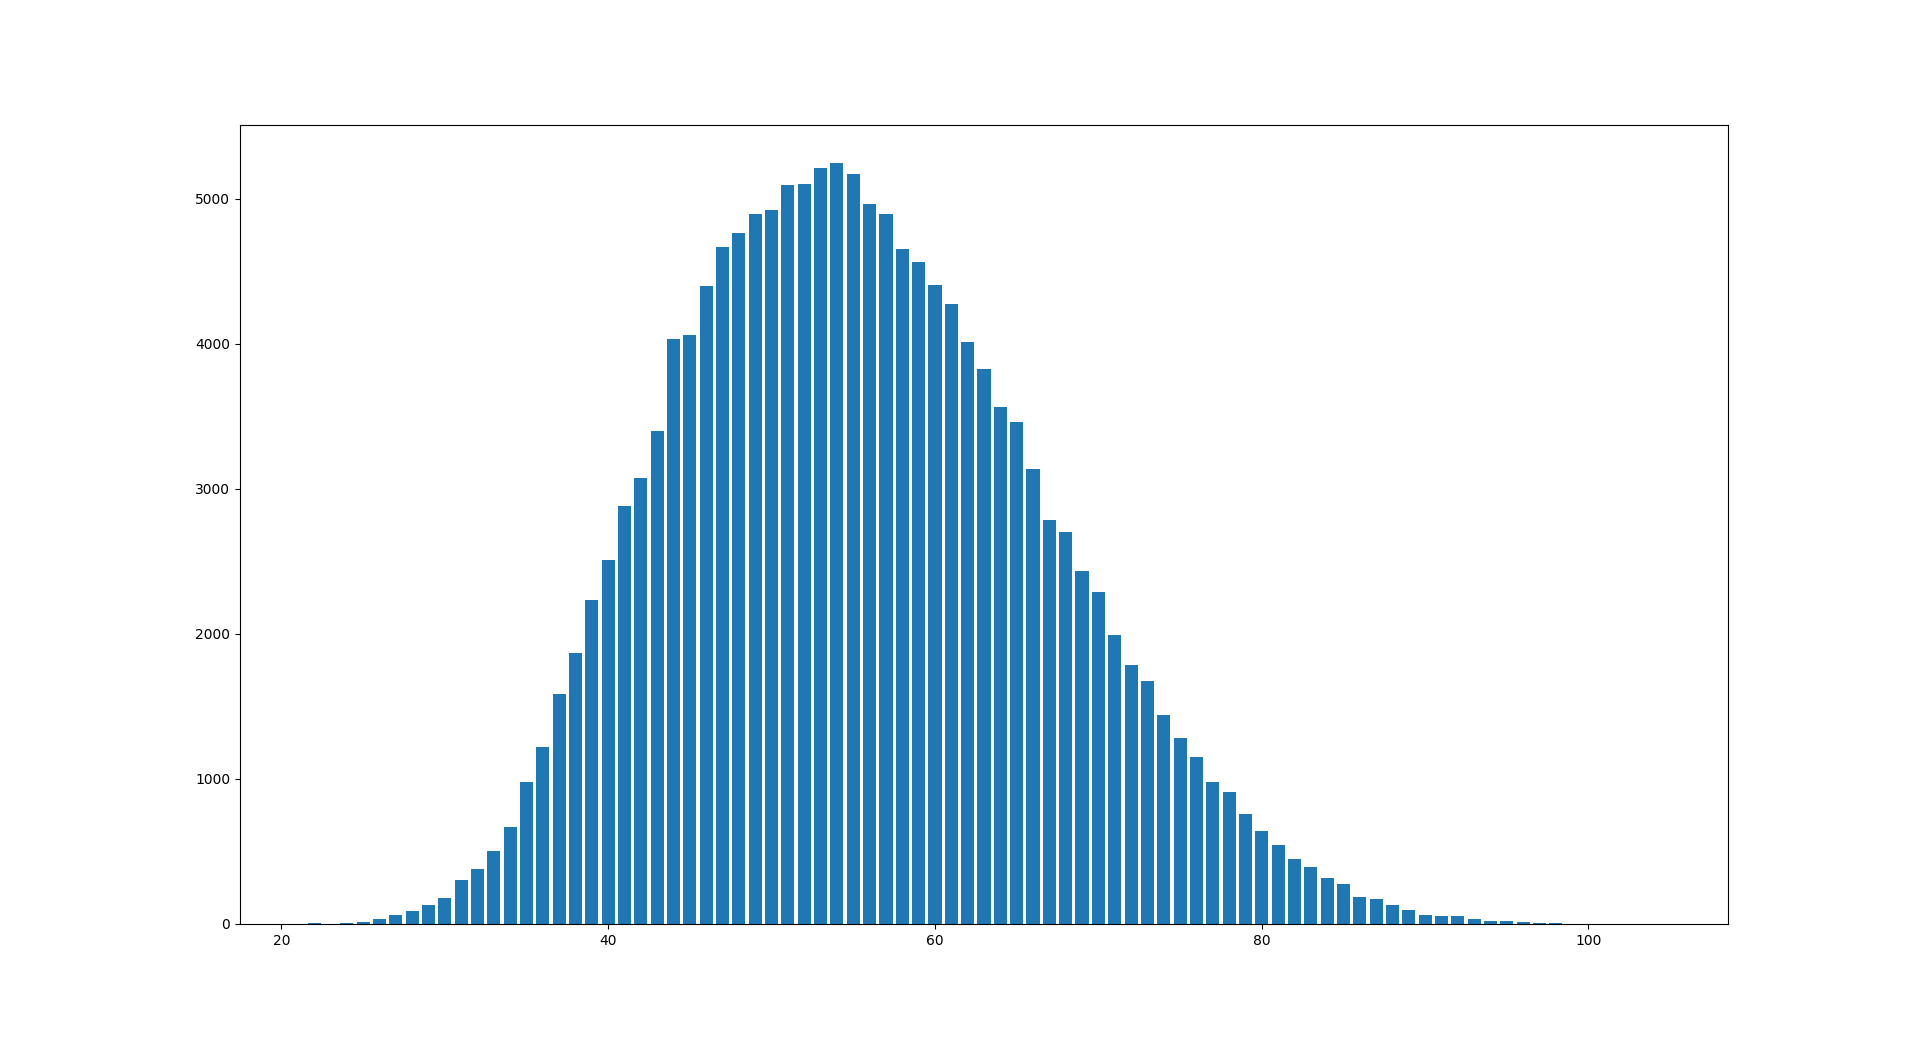
\includegraphics[width=7cm, keepaspectratio]{distribution_of_moves.png}
    \caption{Counts of moves available a random player in 5 games}
    \label{branching_factor}
\end{figure}

As those numbers in isolation are hard to grasp, it is helpful to put Abalone's complexity in relation to other popular games. Its state-space complexity is on the same level as Reversi, whilst its game tree surpasses chess in complexity (c.f. table \ref{complexity_table})

\begin{table}
    \begin{center}
        \begin{tabular}{  c | c | c  }
            Game        & state-space complexity (log) & game-tree complexity (log) \\
            \hline
            \hline
            Tic-tac-toe & 3                            & 5                          \\
            Reversi     & 28                           & 58                         \\
            Chess       & 46                           & 123                        \\
            Abalone     & 24                           & 154                        \\
            Go          & 172                          & 360                        \\
        \end{tabular}
    \end{center}
    \caption{Abalone in comparison with other games \cite{chorus_implementing_2009}}
    \label{complexity_table}
\end{table}

\section{Existing game playing agents}
\label{existing_game_playing_agents}
\subsection{Minimax}
For all the previously discussed methods, game-playing agents based on minimax have been the most successful so far. Heuristic functions are quite similar to those mentioned for chess. Some of the more significant game situations optimized for are:

\begin{itemize}
    \item Adjacency: As a majority of marbles is required to push the opponent's marbles and conversely an equal amount of marbles is needed to avoid being pushed, it can be assumed that keeping one's marbles grouped together is a good move.
    \item Distance to center: Marbles that are close to the brink of the board put them into danger of being attacked, wherefore it is generally good to place all of the marbles into the center of the board. For each player's marbles, we measure their distance from the center of the board as the smallest amount of moves it would take to reach the center (Manhattan distance).
    \item Number of marbles, formation break, single and double marble capturing danger, ... \cite[p. 64]{papadopoulos_exploring_2012}
\end{itemize}

There are multiple implementations of minimax for Abalone \cite{chorus_implementing_2009,lemmens_constructing_2005,ozcan_simple_2004-1,aichholzer_algorithmic_2002}, but software is only openly available for ABA-PRO by Tino Werner from 2002 \cite{aichholzer_oswin_2006}. There are a few mentions of (commercial) Abalone programs like RandomAba (Random Soft), AliAba, AbaloneNet mentioned by Lemmens \cite[p. 7]{lemmens_constructing_2005}, but those have not been attainable through the internet. Even though ABA-PRO was not the strongest algorithm at the time, its availability has made it a frequent benchmark for other papers. Aside from previously mentioned optimizations for minimax like alpha-beta pruning, these programs use more advanced techniques like quiescence search, aspiration windows, and combined move ordering. A more recent publication from 2012 by Papadopoulos et al. claimed to have devised a more successful player. \cite{papadopoulos_exploring_2012}  Those claims could not be confirmed entirely in a recent reimplementation thesis by Michiel Verloop as Papadopoulos' does not describe the weights for the heuristic \cite{verloop_critical_nodate}. This reimplementation in Java \cite{verloop_abaloneai_nodate} is also the reference for later benchmarks as it is open source \cite{verloop_abaloneai_nodate} and thus allows programmatic interaction.

\subsection{MCTS}
The investigations into MCTS in the context of Abalone are pretty limited so far. Pascal Chorus has undertaken a comparison of the vanilla implementation against a heuristic agent, showing the dominance of the heuristic agent. \cite{chorus_implementing_2009} While in games like Go, we don't have loops in Abalone, random players can get stuck in very long games making the results of simulations fragile signals. This approach does not work very well without a more sophisticated rollout policy.

\subsection{Reinforcement Learning}
"Abalearn" was the first learning-based approach to playing Abalone. \cite{campos_abalearn_2003} It was created in 2003 based on temporal difference learning (TD-learning), which is a reinforcement learning method. In the years before, TD-learning had been very successful for backgammon ("TD-Gammon") \cite{tesauro_td-gammon_1994} and for Abalone, the authors achieved to draw ABA-PRO up to a search depth of five. An interesting feature of their approach is that they exclusively used self-play to train the algorithm. Moreover, they introduced a tunable mechanism for making the risk sensitivity of the algorithm dealing with the problem of the agent playing very passively or getting stuck in loops. Modern reinforcement learning methods like Q-learning have only been considered in a smaller project that achieved better than random performance. \cite{mizrachi_introduction_2017}
